\section{Use case model}

\begin{figure}[H]
	\centering
	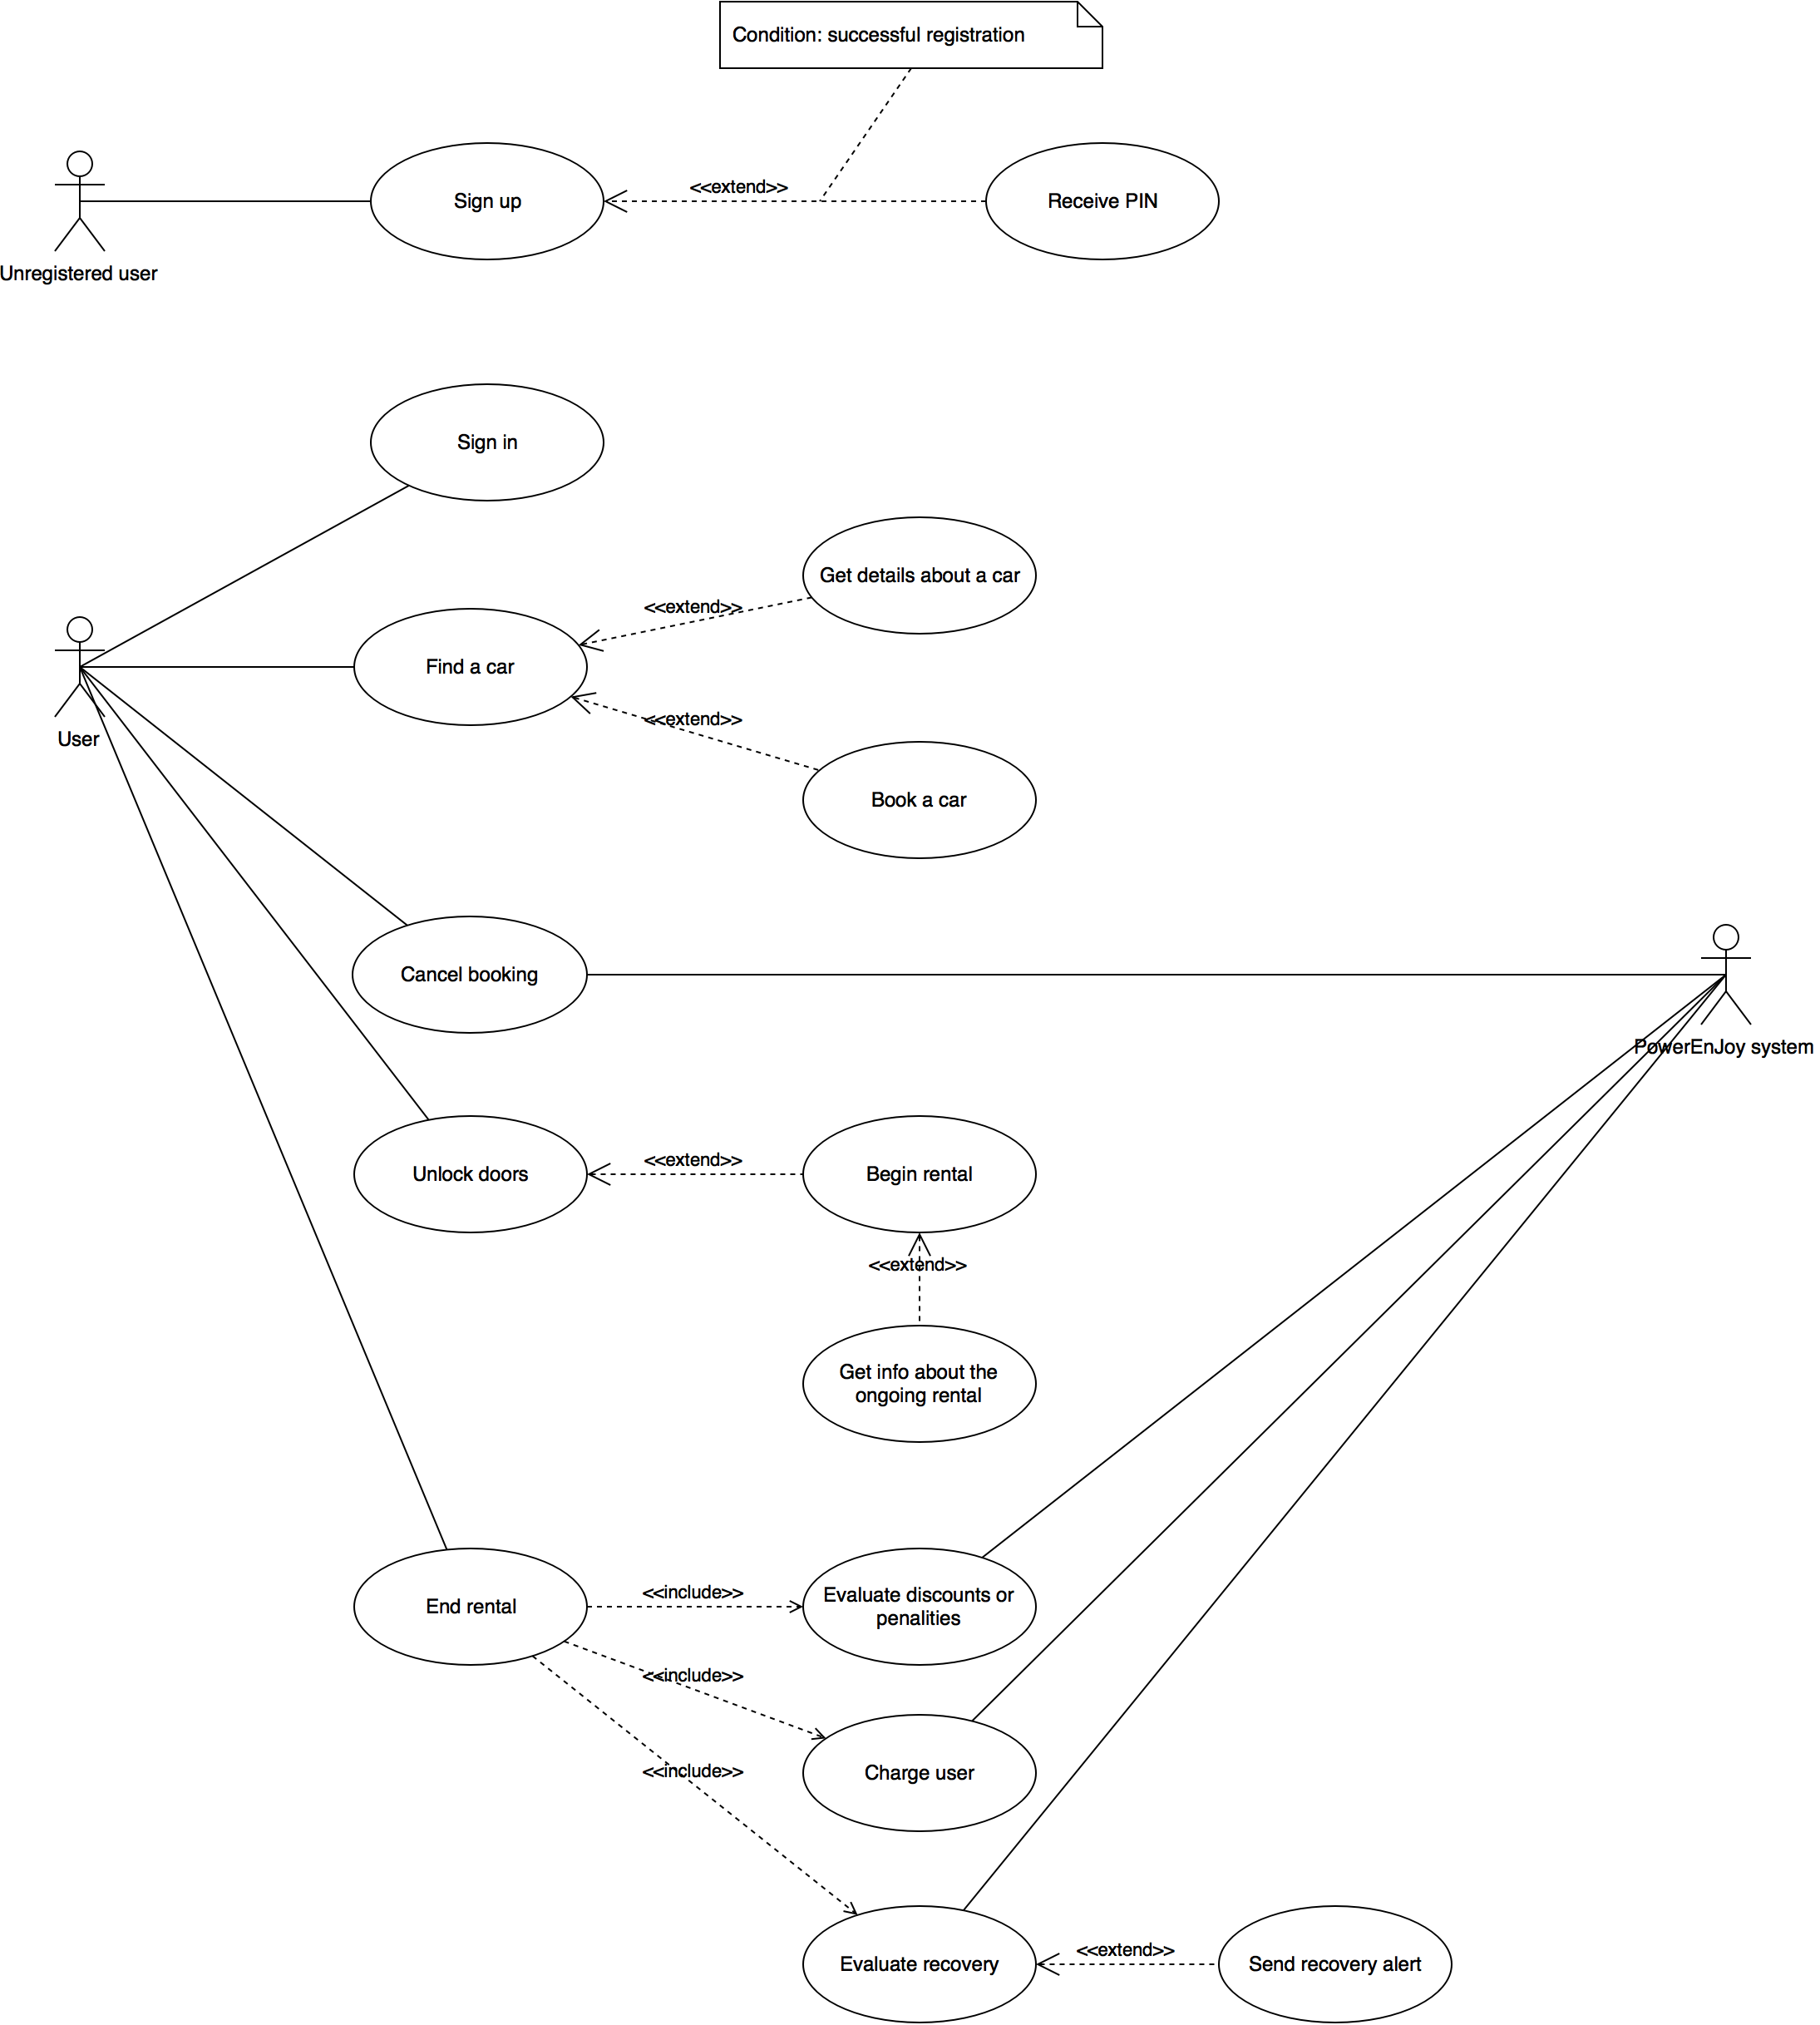
\includegraphics[width=\textwidth]{use-case-model}
	\caption[Use case model]{The diagram above represents the use case model of the PowerEnJoy project. The actors included are the unregistered user, the user and the PowerEnJoy system.}
	\label{fig:use-case-model}
\end{figure}

\subsection{Use case description 1 - Sign up}
\begin{labeling}{use-case-desc-1}
		\item[\textbf{Name}] Sign up
		\item[\textbf{Actors}] User
		\item[\textbf{Entry conditions}] There are no entry conditions.
		\item[\textbf{Flow of events}]
			\begin{itemize}
				\item[]
				\item The user accesses the homepage of PowerEnJoy or opens the app.
				\item The user inserts his/her credentials in the registration form.
				\item The user clicks on the sign up button.
				\item The system processes the registration of the user.
			\end{itemize}
		\item[\textbf{Exit conditions}] The user is successfully registered to the system.
		\item[\textbf{Exceptions}]
			\begin{itemize}
				\item[]
				\item Credentials provided by the user are not correct. In this case the system notifies the user of the error and let him/her to input again his/her credentials. 
				\item User is already registered. In this case the system notifies the user of the impossibility to register.
			\end{itemize}
	\end{labeling}

\subsection{Use case description 2 - Receive the PIN}
\begin{labeling}{use-case-desc-2}
		\item[\textbf{Name}] Receive the PIN
		\item[\textbf{Actors}] User
		\item[\textbf{Entry conditions}] The user must have completed the registration.
		\item[\textbf{Flow of events}]
			\begin{itemize}
				\item[]
				\item The system generates the new PIN for the registered user
				\item The system sends to the registered user his/her PIN via mail
			\end{itemize}
		\item[\textbf{Exit conditions}] The user successfully receives the PIN to use PowerEnJoy cars.
		\item[\textbf{Exceptions}]
			\begin{itemize}
				\item[]
				\item The user doesn’t receive the PIN via mail. In this case the user can ask to the system to send again the mail with the PIN.
			\end{itemize}
	\end{labeling}

\subsection{Use case description 3 - Sign in}
\begin{labeling}{use-case-desc-3}
		\item[\textbf{Name}] Sign in
		\item[\textbf{Actors}] User
		\item[\textbf{Entry conditions}] The user has to be already registered.
		\item[\textbf{Flow of events}]
			\begin{itemize}
				\item[]
				\item The user accesses the homepage of PowerEnJoy or opens the app
				\item The user inputs his email and password
				\item The user clicks on the sign in button
				\item The system redirects the user on his personal page
			\end{itemize}
		\item[\textbf{Exit conditions}] The user is successfully redirected to his personal page.
		\item[\textbf{Exceptions}]
			\begin{itemize}
				\item[]
				\item Email or password provided by the user are not correct. In this case the system notifies the user of the error and let him/her to input again his/her credentials. 
			\end{itemize}
	\end{labeling}
	
\subsection{Use case description 4 - Find a car}
\begin{labeling}{use-case-desc-4}
		\item[\textbf{Name}] Find a car
		\item[\textbf{Actors}] User
		\item[\textbf{Entry conditions}] The user has to be logged in.
		\item[\textbf{Flow of events}]
			\begin{itemize}
				\item[]
				\item The user inserts a specified address or chooses his current position
				\item The system loads on the map all available cars near the position provided by the user
			\end{itemize}
		\item[\textbf{Exit conditions}] The user can see on the map all available cars near the position provided. 
		\item[\textbf{Exceptions}]
			\begin{itemize}
				\item[]
				\item The user inserts an invalid address. In this case the system notifies the user of the error and let him/her to insert a new address.
				\item User’s GPS doesn’t work. In this case the system notifies the user of the impossibility to process the request.
			\end{itemize}
	\end{labeling}
	
\subsection{Use case description 5 - Get details about a car}
\begin{labeling}{use-case-desc-5}
		\item[\textbf{Name}] Get details about a car
		\item[\textbf{Actors}] User
		\item[\textbf{Entry conditions}] The user must have looked for available cars on the map.
		\item[\textbf{Flow of events}]
			\begin{itemize}
				\item[]
				\item The user clicks on an available car shown on the map
				\item The system shows the details about the car chosen by the user
			\end{itemize}
		\item[\textbf{Exit conditions}] The user can see the details of the chosen available car.
		\item[\textbf{Exceptions}]
			\begin{itemize}
				\item[]
				\item Given the assumptions written below, there are no exceptions in this flow of events.
			\end{itemize}
	\end{labeling}	